\documentclass[runningheads]{llncs}
\usepackage[T1]{fontenc}
\usepackage[utf8]{inputenc}
\let\vec\undefined
\usepackage{amsmath}
\usepackage{newtxtext}
\usepackage[varvw]{newtxmath}
\usepackage{graphicx}
\usepackage{tabularx}
\usepackage{array}
\usepackage{url}
\usepackage{microtype}
\usepackage[portuguese]{babel}
\def\UrlBreaks{\do\/\do\-\do\_\do\?\do\&\do\=}
\emergencystretch=2em
\raggedbottom
\setcounter{topnumber}{4}
\setcounter{bottomnumber}{3}
\setcounter{totalnumber}{6}
\renewcommand{\topfraction}{0.95}
\renewcommand{\bottomfraction}{0.9}
\renewcommand{\textfraction}{0.05}
\renewcommand{\floatpagefraction}{0.8}
\setlength{\textfloatsep}{10pt plus 2pt minus 2pt}
\setlength{\floatsep}{8pt plus 2pt minus 2pt}
\setlength{\intextsep}{8pt plus 2pt minus 2pt}
\makeatletter
\setlength{\@fptop}{0pt}
\setlength{\@fpsep}{10pt}
\setlength{\@fpbot}{0pt plus 1fil}
\makeatother
\begin{document}
\renewcommand{\keywordname}{{\bfseries Palavras-chave:}}
\title{Controlo de tráfego e qualidade de serviço em NS-2}
\titlerunning{Controlo de tráfego e QoS em NS-2}
\subtitle{Trabalho Prático 4 -- Qualidade de Serviço na Internet | Grupo 7}

% Identificacao do grupo reproduzida do relatorio de referencia fornecido.
% Os codigos pg... sao identificadores academicos, e nao ORCID.
\author{André Bottari\inst{1} \and David Figueiredo\inst{1} \and Diogo Ferreira\inst{1}}
\authorrunning{}\institute{Departamento de Informática, Universidade do Minho, Portugal\\
\email{pg62400@uminho.pt}\\
\email{pg65402@uminho.pt}\\
\email{pg65406@uminho.pt}}
\maketitle



\begin{abstract}
Comparam-se DropTail, RED e DiffServ numa rede NS-2 de seis clientes e um backbone de 5 Mbps por sentido. Os resultados mostram saturação com seis fontes CBR e exclusão de um fluxo em DropTail sincronizado. RED distribui o débito de forma mais equilibrada sem eliminar as perdas impostas pela sobrecarga UDP. DiffServ protege preferencialmente tráfego conforme; uma proposta com Token Bucket e quatro filas WRR permite preservar 1,5 Mbps por cliente e utilizar capacidade livre nos ensaios realizados.
\keywords{QoS \and NS-2 \and RED \and DiffServ \and Token Bucket}
\end{abstract}

\section{Ambiente e metodologia}
Usou-se NS-2.35 (Debian \texttt{2.35+dfsg-5}) em Docker, substituindo operacionalmente a VM indicada. A--C derivam dos scripts oficiais, preservados em \texttt{originais/files}; C.4 implementa a proposta do grupo. Reproduziu-se a topologia do enunciado~\cite{enunciado}: Cli1--Cli3 (nós 0--2), E1 (3), C0 (4), E2 (5) e Cli4--Cli6 (6--8). Acessos: 5 Mbps/5 ms; backbone: 5 Mbps/10 ms por sentido.

Executaram-se os oito cenários com sementes 7, 11, 23, 41 e 97 (40 execuções). Os gráficos temporais e as primeiras tabelas usam a semente 7; a secção de robustez compara as cinco repetições. A--C geram tráfego em $[0,15[$ s; C.4 em $[0,1;15,1[$ s; terminam aos 16 s. Os gráficos usam intervalos de 1 s e as médias usam $[2,14[$ s. Fixaram-se buffers de 50 pacotes e CBR de 1000 bytes. Corrigiu-se \texttt{packetSize\_} nos CBR e atribuíram-se FIDs distintos ao TCP Tahoe original.

O débito conta bytes recebidos numa única interface; perdas contam descartes nessa fila. O débito no destino conta a última ligação e inclui, em TCP, cabeçalhos e retransmissões: não é goodput. ACKs entram no total da interface e são discriminados nos CSV. Executaram-se também os AWK fornecidos, corrigindo a divisão por zero na janela final de \texttt{bw.awk}. O AWK de perdas agrega toda a rede; os gráficos separam interfaces. Preservaram-se traces, logs, métricas e figuras completas dos dois sentidos. Não se mediram atraso ou jitter.

\section{A -- Best-Effort}
\textbf{A.1.} Cada lado oferece $3\times3=9$ Mbps a um enlace de 5 Mbps. Os gargalos são E1$\to$C0 e E2$\to$C0. C0$\to$E1/E2 recebe tráfego já limitado pelo primeiro gargalo; não se observaram descartes adicionais no core nestes ensaios. As ligações são full duplex: as capacidades nos dois sentidos não se somam para servir o mesmo fluxo.

\textbf{A.2.} Com DropTail, a perda média total aproxima-se de $(9-5)10^6/(1000\times8)=500$ pacotes/s por lado. A chegada periódica e simultânea provoca sincronização e favorece determinados fluxos. No sentido E1$\to$C0, os débitos são 3,000, 2,000 e 0,000 Mbps para Cli1, Cli2 e Cli3. No sentido inverso, Cli4, Cli5 e Cli6 apresentam os mesmos valores. Isto evidencia ausência de justiça entre fluxos; não constitui um resultado universal de qualquer carga DropTail.

\textbf{A.3.} Configurou-se RED apenas nas saídas congestionadas dos edges: limite 50, limiares 10/20 pacotes, $\max_p=0,1$, peso 0,002 e modo \emph{gentle}. O RED aproxima os débitos de 1,667 Mbps por fluxo. O total continua saturado e as perdas mantêm-se próximas de 500 pacotes/s: as fontes UDP não reduzem a taxa em resposta a descartes antecipados. Não foram medidas latência ou jitter; não se infere melhoria dessas métricas apenas destes gráficos.
\begin{table}[htbp]\centering\small
\caption{Débitos por fluxo em Mbps e perdas totais; médias em $[2,14[$ s. Em C, F1 e F6 são os clientes protegidos.}
\begin{tabular}{llllll}\hline
Cenário & Ligação & F1/F4 & F2/F5 & F3/F6 & Perdas/s\\\hline
A\_droptail & 3$\to$4 & 3,000 & 2,000 & 0,000 & 499,917\\
A\_droptail & 5$\to$4 & 3,000 & 2,000 & 0,000 & 499,917\\
A\_red & 3$\to$4 & 1,667 & 1,665 & 1,668 & 499,833\\
A\_red & 5$\to$4 & 1,673 & 1,652 & 1,675 & 500,250\\
C\_diffserv & 3$\to$4 & 2,438 & 1,309 & 1,253 & 500,000\\
C\_diffserv & 5$\to$4 & 1,296 & 1,296 & 2,408 & 499,917\\
\hline\end{tabular}\end{table}
\begin{figure}[!htbp]\centering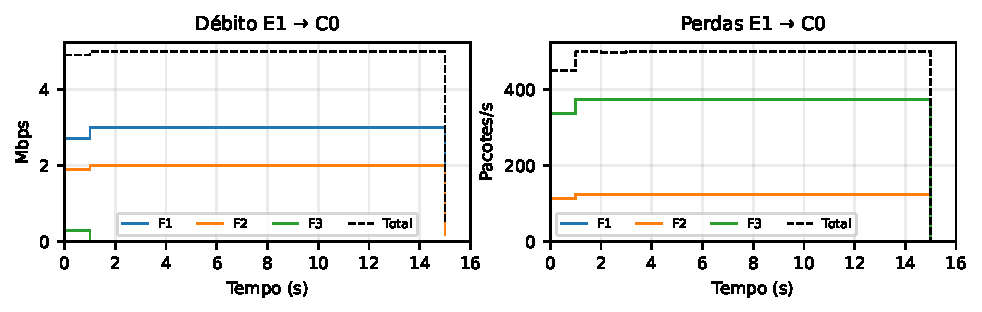
\includegraphics[width=\textwidth]{../figuras/A_droptail_compacto.pdf}\caption{A.2: DropTail, débito e perdas em E1$\to$C0; fluxos 1--3. O sentido inverso apresenta o mesmo padrão.}\label{fig:A_droptail}\end{figure}
\begin{figure}[!htbp]\centering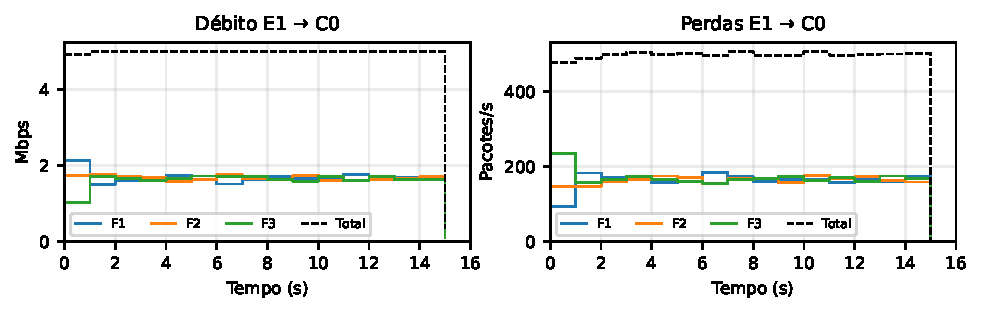
\includegraphics[width=\textwidth]{../figuras/A_red_compacto.pdf}\caption{A.3: RED em E1$\to$C0. A repartição melhora mantendo-se o congestionamento.}\label{fig:A_red}\end{figure}

\section{B -- Aplicações heterogéneas}
Instalaram-se CBR Cli1$\leftrightarrow$Cli6 (3 Mbps, 1000 bytes), FTP/TCP Cli2$\to$Cli5 e Cli4$\to$Cli2, e voz Cli3$\leftrightarrow$Cli4 (160 bytes, 64 kbps durante atividade). Preservou-se o modelo exponencial do procedimento fornecido: conversa média de 0,4 s e silêncio de 1,0 s; a taxa média de longo prazo esperada é cerca de 18,3 kbps. Esta configuração da voz é uma escolha experimental, pois o enunciado não fixa esses valores.

\textbf{B.1.} Na configuração original com janela TCP máxima de 20 pacotes, cenário de referência, não se observaram perdas. Cada FTP recebe cerca de 1,883 Mbps. Para estudar efetivamente a competição sob congestionamento, realizou-se \texttt{B\_misto}, com janela TCP máxima de 128 pacotes e restantes parâmetros mantidos. As perdas passam a afetar dados e ACKs; os FTP reduzem os débitos médios para 1,724 e 1,471 Mbps. O tráfego CBR mantém a oferta próxima de 3 Mbps e recebe 2,963/2,984 Mbps nos destinos. O TCP reage à congestão e à perda de ACKs, diminuindo a janela e retransmitindo; por isso sofre maior redução de débito neste ensaio. A voz perde menos pacotes em valor absoluto, mas a perda não é recuperada pela aplicação UDP e pode degradar a conversação. Não se compara qualidade de voz apenas com contagens absolutas, A análise entre sementes apresentada adiante avalia a variabilidade; outras taxas exigem novos ensaios.
\begin{table}[htbp]\centering\small
\caption{B: débito recebido no destino em Mbps e perdas de dados na entrada do backbone no cenário com janela 128.}
\begin{tabular}{llll}\hline
Aplicação & Janela 20 & Janela 128 & Perdas dados/s\\\hline
CBR 1--6 & 2,995 & 2,963 & 3,417\\
FTP 2--5 & 1,883 & 1,724 & 0,583\\
Voz 3--4 & 0,021 & 0,021 & 0,083\\
CBR 6--1 & 2,996 & 2,984 & 1,667\\
FTP 4--2 & 1,883 & 1,471 & 1,417\\
Voz 4--3 & 0,021 & 0,020 & 0,250\\
\hline\end{tabular}\end{table}
\begin{figure}[!htbp]\centering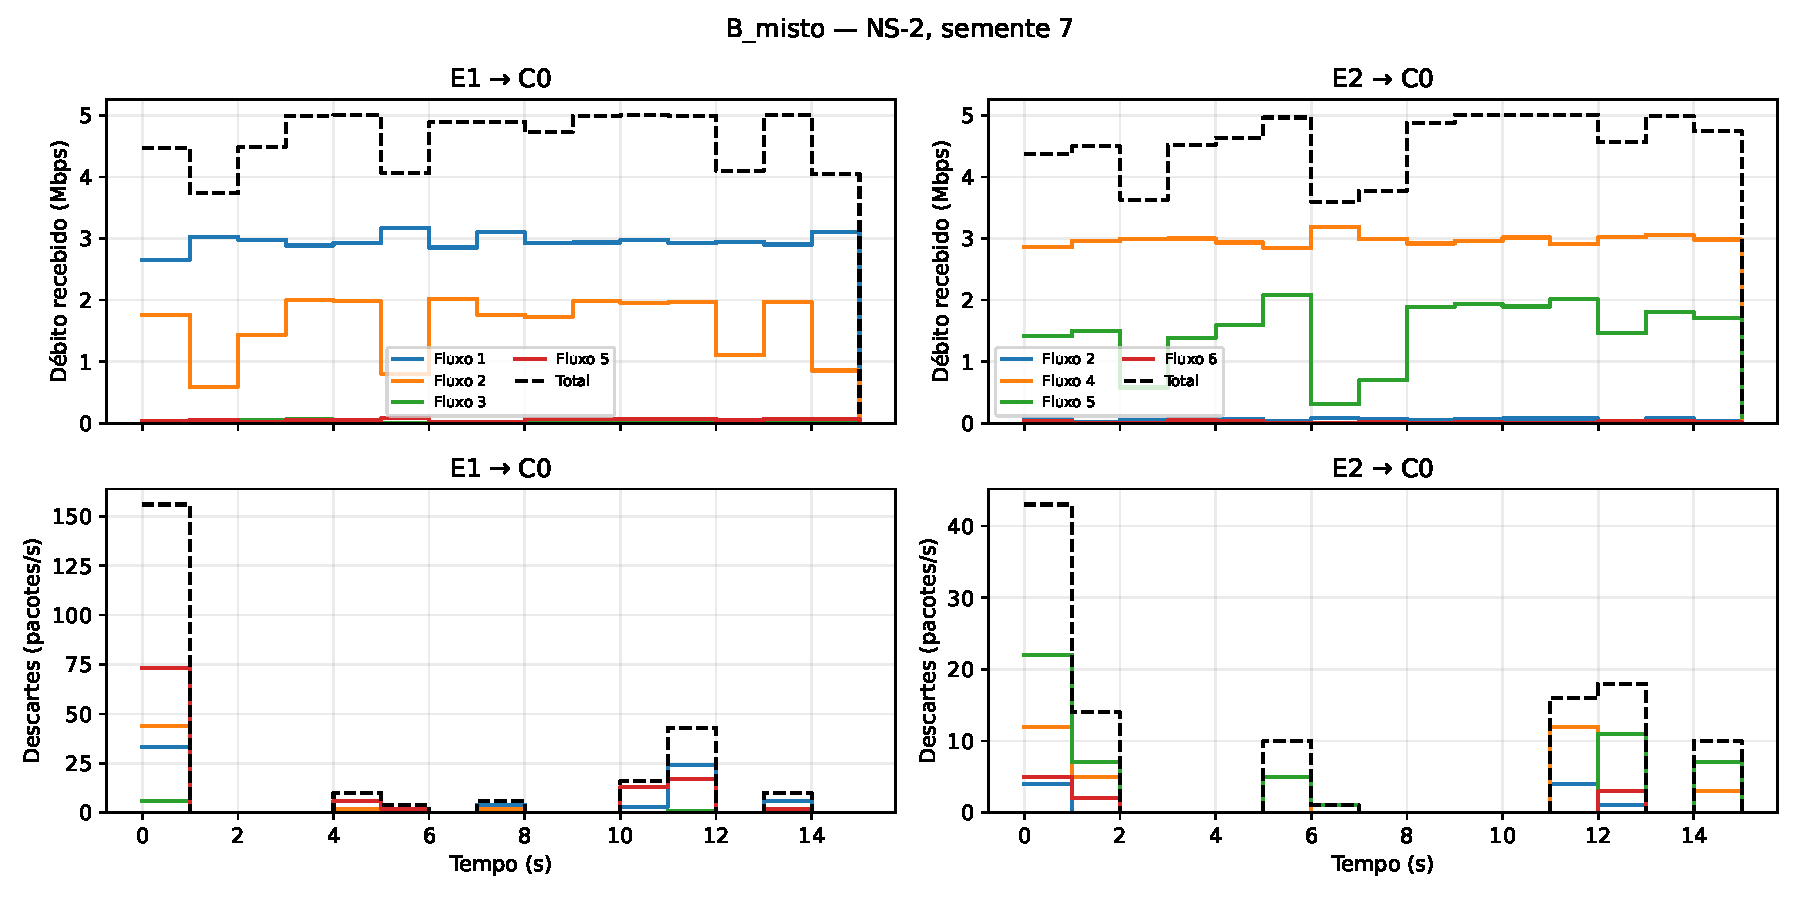
\includegraphics[width=\textwidth]{../figuras/B_misto.pdf}\caption{B: aplicações heterogéneas, janela TCP 128. As curvas dos fluxos TCP incluem os respetivos ACKs no sentido contrário.}\label{fig:B_misto}\end{figure}

\section{C -- Differentiated Services}
\textbf{C.1.} A inspeção de \texttt{qos1.tcl} confirma uma fila física (0), duas precedências virtuais de descarte (0/1) e RR por defeito. Só existe uma fila física ativa, logo o agendamento RR não reparte capacidade entre clientes. Usa-se RIO-C~\cite{manual}: para CP10 considera-se a ocupação conforme; para CP11, a ocupação agregada. O limite é 50 pacotes por fila física, partilhado pelas precedências. Para pacotes de 1000 bytes representa capacidade nominal de 50\,000 bytes de pacotes; não representa a memória real do processo NS-2, que contém estruturas e metadados. O código de implementação confirma que o limite é atribuído a cada fila física~\cite{codigo}.

O edge E1 mede Cli1$\to$Cli6 com Token Bucket (CIR 2 Mbps, CBS 5000 bytes); o conforme recebe CP10 e o excedente CP11. A política \texttt{Dumb} com origem/destino \texttt{-1} marca todo o restante tráfego CP11 (o simulador apresenta-a como Null). E2 protege simetricamente Cli6$\to$Cli1. O core preserva o mapeamento CP10/CP11 para a mesma fila física.
\begin{table}[htbp]\centering\small
\caption{Configuração RIO-C original em cada interface DiffServ.}
\begin{tabular}{llllll}\hline
CP & Fila física & Precedência & $\min_{th}$ & $\max_{th}$ & $\max_p$\\\hline
10 & 0 & 0 & 20 & 40 & 0,02\\
11 & 0 & 1 & 10 & 20 & 0,10\\
\hline\end{tabular}\end{table}

\textbf{C.2.} A precedência CP11 concentra a perda. No final da simulação, E1$\to$C0 recebe 3754 pacotes CP10 sem descarte; CP11 recebe 13\,124 e perde 6252 por limite mais 1235 antecipadamente (7487, ou 57,05\%). Em E2$\to$C0, CP11 perde 7415 de 13\,124 (56,50\%), mas CP10 também perde 71 de 3754 (1,89\%) por limite. Logo, a proteção de descarte não impede perdas conformes quando o buffer físico partilhado está cheio. As saídas do core não registam perdas. Estes contadores cobrem toda a execução, enquanto as médias da tabela cobrem apenas $[2,14[$ s.

\textbf{C.3.} Cli1$\to$Cli6 obtém 2,438 Mbps na interface E1$\to$C0, e os restantes fluxos desse lado 1,309 e 1,253 Mbps. No sentido inverso, o cliente protegido obtém 2,408 Mbps, contra 1,296 Mbps para cada outro. A classificação privilegia o contrato, ao contrário do RED indiferenciado, mas não aumenta os 5 Mbps totais. O cliente protegido pode receber mais que o CIR porque parte do excedente CP11 também é transmitida. Não se trata de garantia rígida de 2 Mbps nem de justiça igual entre todos os clientes.
\begin{figure}[!htbp]\centering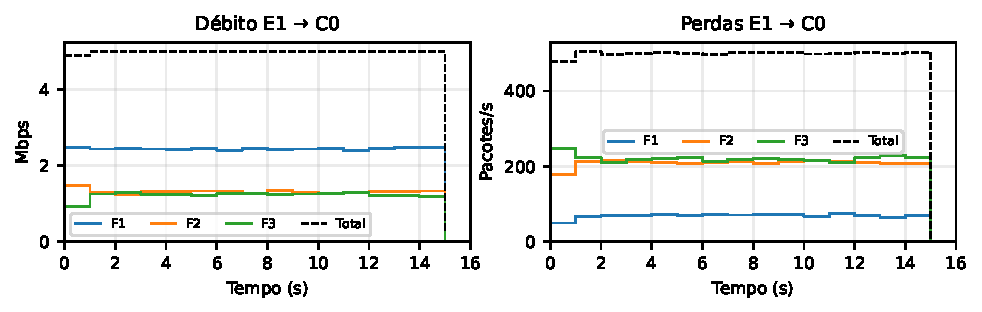
\includegraphics[width=\textwidth]{../figuras/C_diffserv_compacto.pdf}\caption{C.3: DiffServ em E1$\to$C0; o fluxo protegido é F1. O sentido inverso consta das séries e tabelas.}\label{fig:C_diffserv}\end{figure}


\section{C.4 -- Política de 30\% por cliente}
A quota é $0,30\times5=1,5$ Mbps por cliente e sentido; os três contratos somam 4,5 Mbps. Cada cliente recebe um Token Bucket próprio (CIR 1,5 Mbps, CBS 5000 bytes). Pacotes conformes recebem CP10, CP20 ou CP30, e todos os excedentes são remarcados CP11. Em cada interface do backbone usam-se quatro filas físicas com WRR $3:3:3:1$. Para pacotes iguais e quatro filas saturadas, cada classe conforme recebe 30\% das oportunidades de transmissão e o excedente recebe 10\%. O excedente é encaminhado numa classe de menor peso; esta é uma prioridade relativa de serviço, não prioridade estrita PRI. Filas vazias cedem oportunidades, permitindo aproveitar capacidade livre.
\begin{table}[htbp]\centering\small
\caption{Política proposta, igual nos edges e core. Cada fila tem limite de 50 pacotes.}
\begin{tabular}{lllll}\hline
Classe & CP & Fila & Peso & RED (min, max, p)\\\hline
Cliente A conforme & 10 & 0 & 3 & 20; 40; 0,02\\
Cliente B conforme & 20 & 1 & 3 & 20; 40; 0,02\\
Cliente C conforme & 30 & 2 & 3 & 20; 40; 0,02\\
Excedentes & 11 & 3 & 1 & 10; 20; 0,10\\
\hline\end{tabular}\end{table}

\textbf{Validação.} Executaram-se três cargas simétricas: normal (três clientes a 3 Mbps por lado), livre (um cliente a 5 Mbps por lado) e abuso (um a 4,5 Mbps e dois a 1,5 Mbps). A tabela apresenta as receções nos destinos, e a figura conjunta mostra E1$\to$C0. Os gráficos completos dos dois sentidos acompanham os ficheiros do projeto. Nos ensaios normal e abuso, todas as classes conformes apresentam zero descartes nas quatro interfaces; as perdas concentram-se em CP11. A remarcação está comprovada pelos contadores CP11: em E1$\to$C0 no caso normal foram classificados 8427 pacotes excedentes, dos quais 955 aceites e 7472 descartados. Os contadores \texttt{TxPkts} representam aceitação na fila, não receção no destino.
\begin{table}[htbp]\centering\small
\caption{C.4: débito nos destinos (Mbps). A/B/C designam a ordem das três fontes em cada lado, não os FIDs de A--C.}
\begin{tabular}{lllll}\hline
Carga & Origem & Cliente A & Cliente B & Cliente C\\\hline
C4\_normal & E1 & 1,733 & 1,638 & 1,629\\
C4\_normal & E2 & 1,723 & 1,641 & 1,636\\
C4\_livre & E1 & 5,000 & inativo & inativo\\
C4\_livre & E2 & 5,000 & inativo & inativo\\
C4\_abuso & E1 & 2,000 & 1,500 & 1,500\\
C4\_abuso & E2 & 2,000 & 1,500 & 1,500\\
\hline\end{tabular}\end{table}

O caso normal entrega pelo menos 1,629 Mbps a cada cliente; livre entrega 5 Mbps ao único cliente ativo; abuso limita a vantagem do cliente agressivo a 2 Mbps e preserva 1,5 Mbps para cada outro. Estes ensaios ilustram proteção e empréstimo; não demonstram garantia universal para outras rajadas ou tamanhos de pacote.

\textbf{Perspetiva do ISP.} A proposta protege contratos e aproveita capacidade livre, mas exige admissão e policiamento agregado por cliente. WRR reparte pacotes; tamanhos diferentes podem distorcer quotas em bits/s, exigindo justiça em bytes. A separação conforme/excedente pode reordenar pacotes. C.4 usa quatro buffers de 50 pacotes contra um em C, alterando também o armazenamento. Outras rajadas podem causar perdas conformes; garantias fim a fim exigem dimensionamento de todo o percurso.
\begin{figure}[!htbp]\centering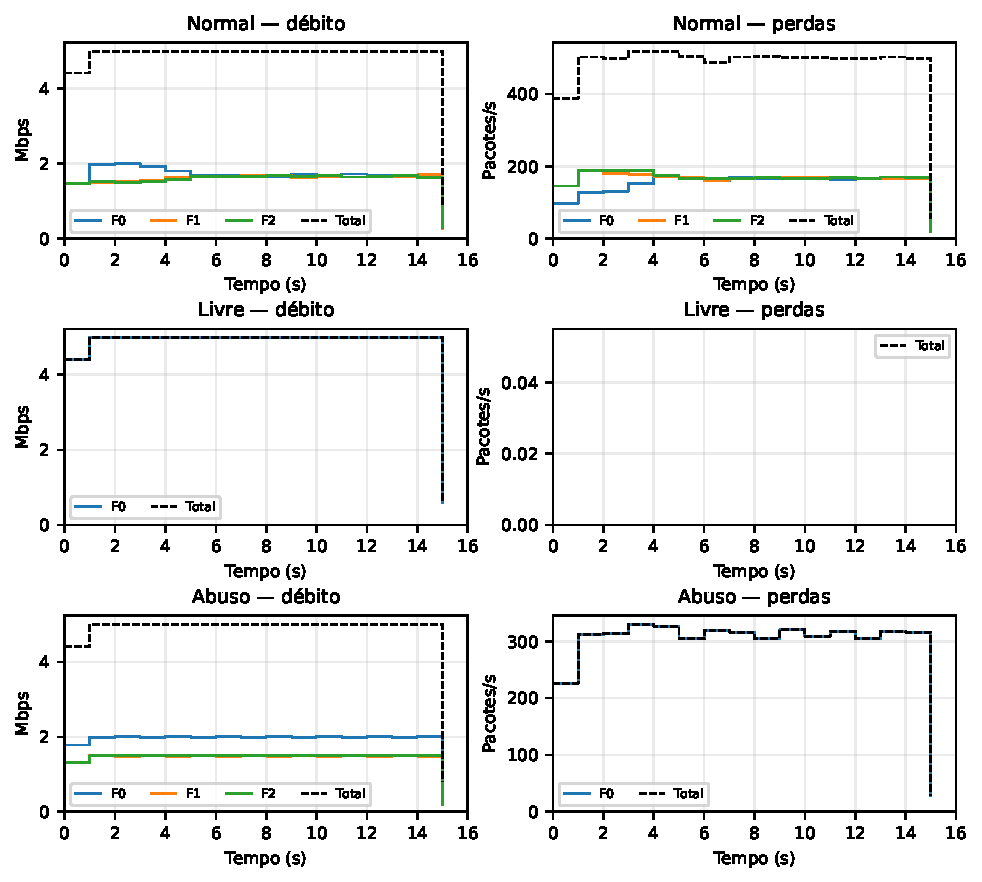
\includegraphics[width=\textwidth]{../figuras/C4_comparacao.pdf}\caption{C.4: débito e perdas em E1$\to$C0, semente 7. Normal: três fontes a 3 Mbps; livre: uma a 5 Mbps; abuso: 4,5/1,5/1,5 Mbps. FIDs 0--2.}\label{fig:C4_comparacao}\end{figure}

\section{Robustez entre sementes}
A tabela resume cinco médias temporais em $[2,14[$ s: média, desvio-padrão amostral ($n-1$) e mínimo--máximo observado, não intervalos de confiança. Traces e métricas constam de \texttt{resultados/multissementes}.
\begin{table}[htbp]\centering\small
\caption{Débitos nas cinco sementes (Mbps); em C.4, mínimo entre os seis clientes por execução.}
\begin{tabular}{lll}\hline
Indicador & Média $\pm$ desvio & Mínimo--máximo\\\hline
RED: F1, interface & 1,661$\,\pm\,$0,020 & 1,642--1,693\\
FTP 2--5, janela 20 & 1,881$\,\pm\,$0,002 & 1,879--1,883\\
FTP 2--5, janela 128 & 1,553$\,\pm\,$0,122 & 1,423--1,724\\
FTP 4--2, janela 128 & 1,561$\,\pm\,$0,076 & 1,471--1,630\\
DiffServ: Cli1--Cli6 & 2,427$\,\pm\,$0,013 & 2,411--2,439\\
DiffServ: Cli6--Cli1 & 2,409$\,\pm\,$0,016 & 2,383--2,423\\
C.4 normal: mínimo & 1,627$\,\pm\,$0,002 & 1,624--1,629\\
C.4 abuso: mínimo & 1,500$\,\pm\,$0,000 & 1,500--1,500\\
\hline\end{tabular}\end{table}

DropTail mantém 3/2/0 Mbps nas cinco sementes: mudar a semente não altera esta carga determinística nem explora outras fases de chegada. RED mantém perdas entre 499,667 e 500,500 pacotes/s por interface, confirmando saturação e repartição mais equilibrada. DiffServ preserva a vantagem dos clientes protegidos.

Os FTP congestionados recebem em média 1,553 e 1,561 Mbps, invertendo a ordem entre sentidos em algumas sementes. Confirma-se a redução face à janela 20, sem evidência de um sentido sistematicamente mais prejudicado. A voz aleatória e a dinâmica TCP contribuem para a variabilidade.

Em C.4, o mínimo entre clientes e sementes é 1,624 Mbps na carga normal e 1,500 Mbps em abuso. O caso livre mantém 5 Mbps nos dois sentidos. Não há perdas conformes em normal/abuso, e as 40 execuções passam conservação UDP e capacidade.

\section{Conclusão}
DropTail pode excluir fluxos sincronizados; RED equilibra a repartição sem eliminar a sobreoferta UDP. DiffServ protege preferencialmente tráfego contratado. Token Bucket com WRR preserva quotas e permite empréstimo nas cinco sementes. As conclusões restringem-se às cargas testadas; outras rajadas, fases e tamanhos de pacote exigem validação adicional.

\begin{thebibliography}{3}
\bibitem{enunciado} Universidade do Minho: TP4 -- Estudo de QoS e Mecanismos de Controlo de Tráfego. QoSI, 2026/2027. Enunciado e scripts disponibilizados na unidade curricular.
\bibitem{manual} The ns Manual: Differentiated Services -- Configuration. \url{https://www.isi.edu/websites/nsnam/ns/doc/node97.html}
\bibitem{codigo} NS-2.35: implementação de \texttt{dsREDQueue} e \texttt{redQueue}. \url{https://github.com/hbatmit/ns2.35/tree/master/diffserv}
\end{thebibliography}
\end{document}
